% Options for packages loaded elsewhere
\PassOptionsToPackage{unicode}{hyperref}
\PassOptionsToPackage{hyphens}{url}
%
\documentclass[
]{article}
\usepackage{amsmath,amssymb}
\usepackage{iftex}
\ifPDFTeX
  \usepackage[T1]{fontenc}
  \usepackage[utf8]{inputenc}
  \usepackage{textcomp} % provide euro and other symbols
\else % if luatex or xetex
  \usepackage{unicode-math} % this also loads fontspec
  \defaultfontfeatures{Scale=MatchLowercase}
  \defaultfontfeatures[\rmfamily]{Ligatures=TeX,Scale=1}
\fi
\usepackage{lmodern}
\ifPDFTeX\else
  % xetex/luatex font selection
\fi
% Use upquote if available, for straight quotes in verbatim environments
\IfFileExists{upquote.sty}{\usepackage{upquote}}{}
\IfFileExists{microtype.sty}{% use microtype if available
  \usepackage[]{microtype}
  \UseMicrotypeSet[protrusion]{basicmath} % disable protrusion for tt fonts
}{}
\makeatletter
\@ifundefined{KOMAClassName}{% if non-KOMA class
  \IfFileExists{parskip.sty}{%
    \usepackage{parskip}
  }{% else
    \setlength{\parindent}{0pt}
    \setlength{\parskip}{6pt plus 2pt minus 1pt}}
}{% if KOMA class
  \KOMAoptions{parskip=half}}
\makeatother
\usepackage{xcolor}
\usepackage[margin=1in]{geometry}
\usepackage{graphicx}
\makeatletter
\def\maxwidth{\ifdim\Gin@nat@width>\linewidth\linewidth\else\Gin@nat@width\fi}
\def\maxheight{\ifdim\Gin@nat@height>\textheight\textheight\else\Gin@nat@height\fi}
\makeatother
% Scale images if necessary, so that they will not overflow the page
% margins by default, and it is still possible to overwrite the defaults
% using explicit options in \includegraphics[width, height, ...]{}
\setkeys{Gin}{width=\maxwidth,height=\maxheight,keepaspectratio}
% Set default figure placement to htbp
\makeatletter
\def\fps@figure{htbp}
\makeatother
\setlength{\emergencystretch}{3em} % prevent overfull lines
\providecommand{\tightlist}{%
  \setlength{\itemsep}{0pt}\setlength{\parskip}{0pt}}
\setcounter{secnumdepth}{-\maxdimen} % remove section numbering

%\newcommand{\beginsupplement}{%
%        \setcounter{table}{0}
%        \renewcommand{\thetable}{\arabic{table}}%
%        \setcounter{figure}{0}
%        \renewcommand{\thefigure}{\arabic{figure}}%
%     }

\newcommand{\beginsupplement}{
	\renewcommand{\figurename}{Supplementary Figure}
	\setcounter{figure}{0}
}

%\usepackage{xr}
%\externaldocument{Supplementary_File1}

\usepackage{lineno}
\linenumbers

\usepackage[compress, super]{natbib}

\usepackage{setspace} \doublespacing

\usepackage{siunitx}

\usepackage[utf8]{inputenc}
\usepackage{amsmath}
\usepackage{algorithm}
\usepackage{algpseudocode}

\algrenewcommand\algorithmicrequire{\textbf{Input:}}
\algrenewcommand\algorithmicensure{\textbf{Output:}}
\ifLuaTeX
  \usepackage{selnolig}  % disable illegal ligatures
\fi
\IfFileExists{bookmark.sty}{\usepackage{bookmark}}{\usepackage{hyperref}}
\IfFileExists{xurl.sty}{\usepackage{xurl}}{} % add URL line breaks if available
\urlstyle{same}
\hypersetup{
  pdftitle={Compiled Figures for: Transcripts with high distal heritability mediate genetic effects on complex metabolic traits},
  hidelinks,
  pdfcreator={LaTeX via pandoc}}

\title{Compiled Figures for: Transcripts with high distal heritability
mediate genetic effects on complex metabolic traits}
\author{}
\date{\vspace{-2.5em}}

\begin{document}
\maketitle

\begin{figure}[ht!]
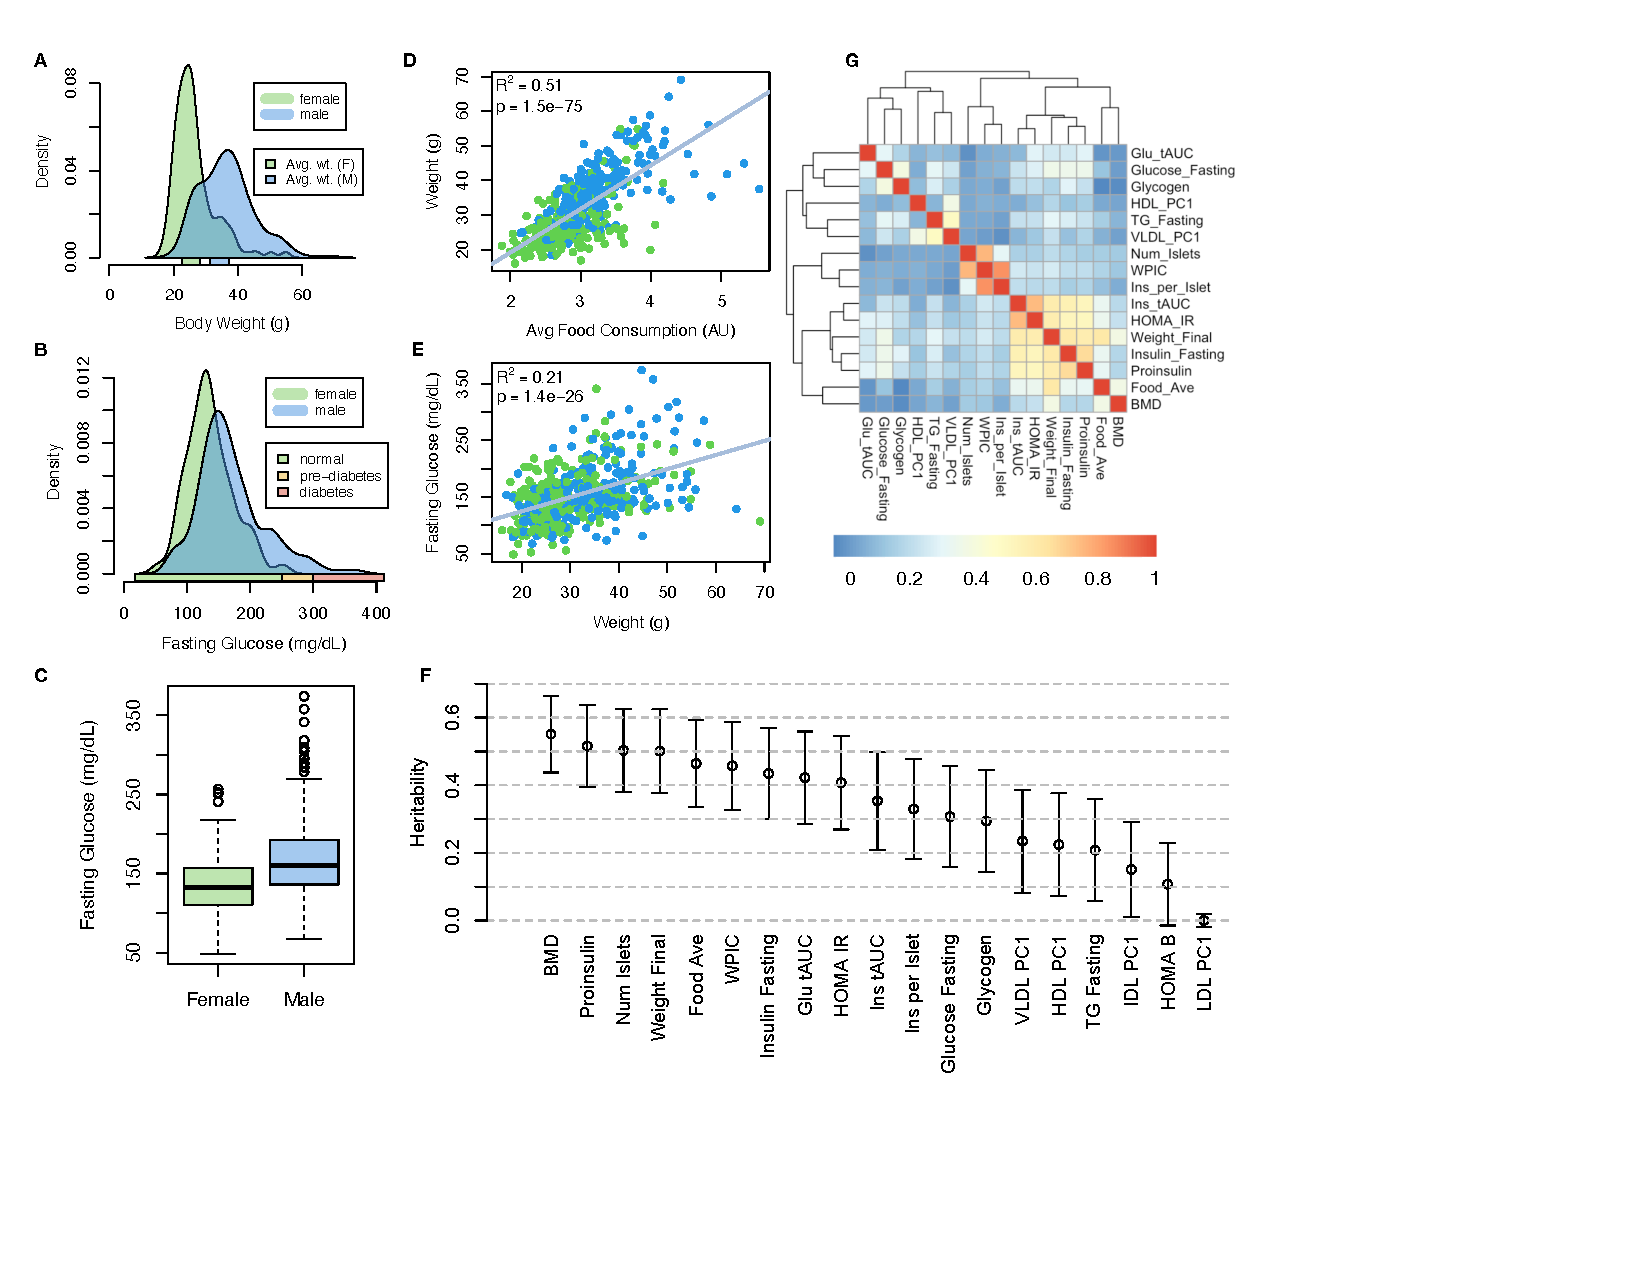
\includegraphics[width=\textwidth]{Figures/Fig1_trait_overview.pdf} 
\caption{Clinical overview. \textbf{A.} Distributions of final body 
weight in female (green) and male (blue) diversity outbred mice.
The average B6 female and male adult weights at 24 weeks of 
age are indicated by green and blue bars respectively on the 
$x$-axis. \textbf{B.} Distributions of fasting glucose in female 
(green) and male (blue) DO mice. Normal (green), pre-diabetic
(yellow), and diabetic (red) fasting glucose ranges for mice are 
shown by colored bars along the $x$-axis. \textbf{C.} Males 
(blue $n = 242$) had higher fasting blood glucose on average 
(mean = 170.0 mg/dL) than females (green $n = 240$, 
mean = 136) (two-sided Welch's t test: $t = 8.02$, 
df = 428.9, 95\% CI of difference = 25.4 to 42.0 mg/dL; 
$p = 1.05\times10^{-14}$). Lines in boxes 
correspond to the median; lower and upper edges of 
boxes indicate the first and third quartiles; whiskers 
indicate the first and third quartiles $\pm$ 1.5 times
the interquartile range; dots indicate outliers beyond 1.5 times
the interquartile range. \textbf{D.} The relationship between 
food consumption and body weight for female (green) and 
male (blue) DO mice. (Linear regression 
$R^2 = 0.51$;  beta coefficient = $12.6\pm0.57$ 
standard error; $t = 22.2$; $p < 2.2^{-16}$). \textbf{E.} 
Relationship between body weight and fasting glucose for 
female (green) and male (blue) DO mice. (Linear regression 
$R^2 = 0.21$; beta coefficient = $2.49\pm 0.22$ 
standard error; $t = 11.34$; $p < 2.2^{-16}$). In D and E,
blue lines show line of best fit. \textbf{F.} Data 
presented are heritability estimates for each physiological trait. 
Bars show standard error of each estimate. The number of animals 
used in each estimate is shown in parentheses after each trait name. 
\textbf{G.} Correlation structure between pairs of physiological 
traits. The upper and lower triangle show the Pearson correlation 
coefficients ($r$) between LOD traces of trait pairs (blue) and trait 
pairs (purple) respectively. The diagonal (orange) shows the estimated 
heritability of each trait. BMD - bone mineral density, WPIC - whole 
pancreas insulin content, Glu tAUC - glucose total area under the 
curve, HOMA IR - homeostatic measurement of insulin resistance, 
HOMA B - homeostatic measure of beta cell health, VLDL - very 
low-density lipoprotein, LDL - low-density lipoprotein, IDL - intermediate 
density lipoprotein, HDL - high-density lipoprotein, TG - triglyceride. 
Source data are provided as a Source Data file.
}
\label{fig:trait_overview}
\end{figure}

\begin{figure}[ht!]
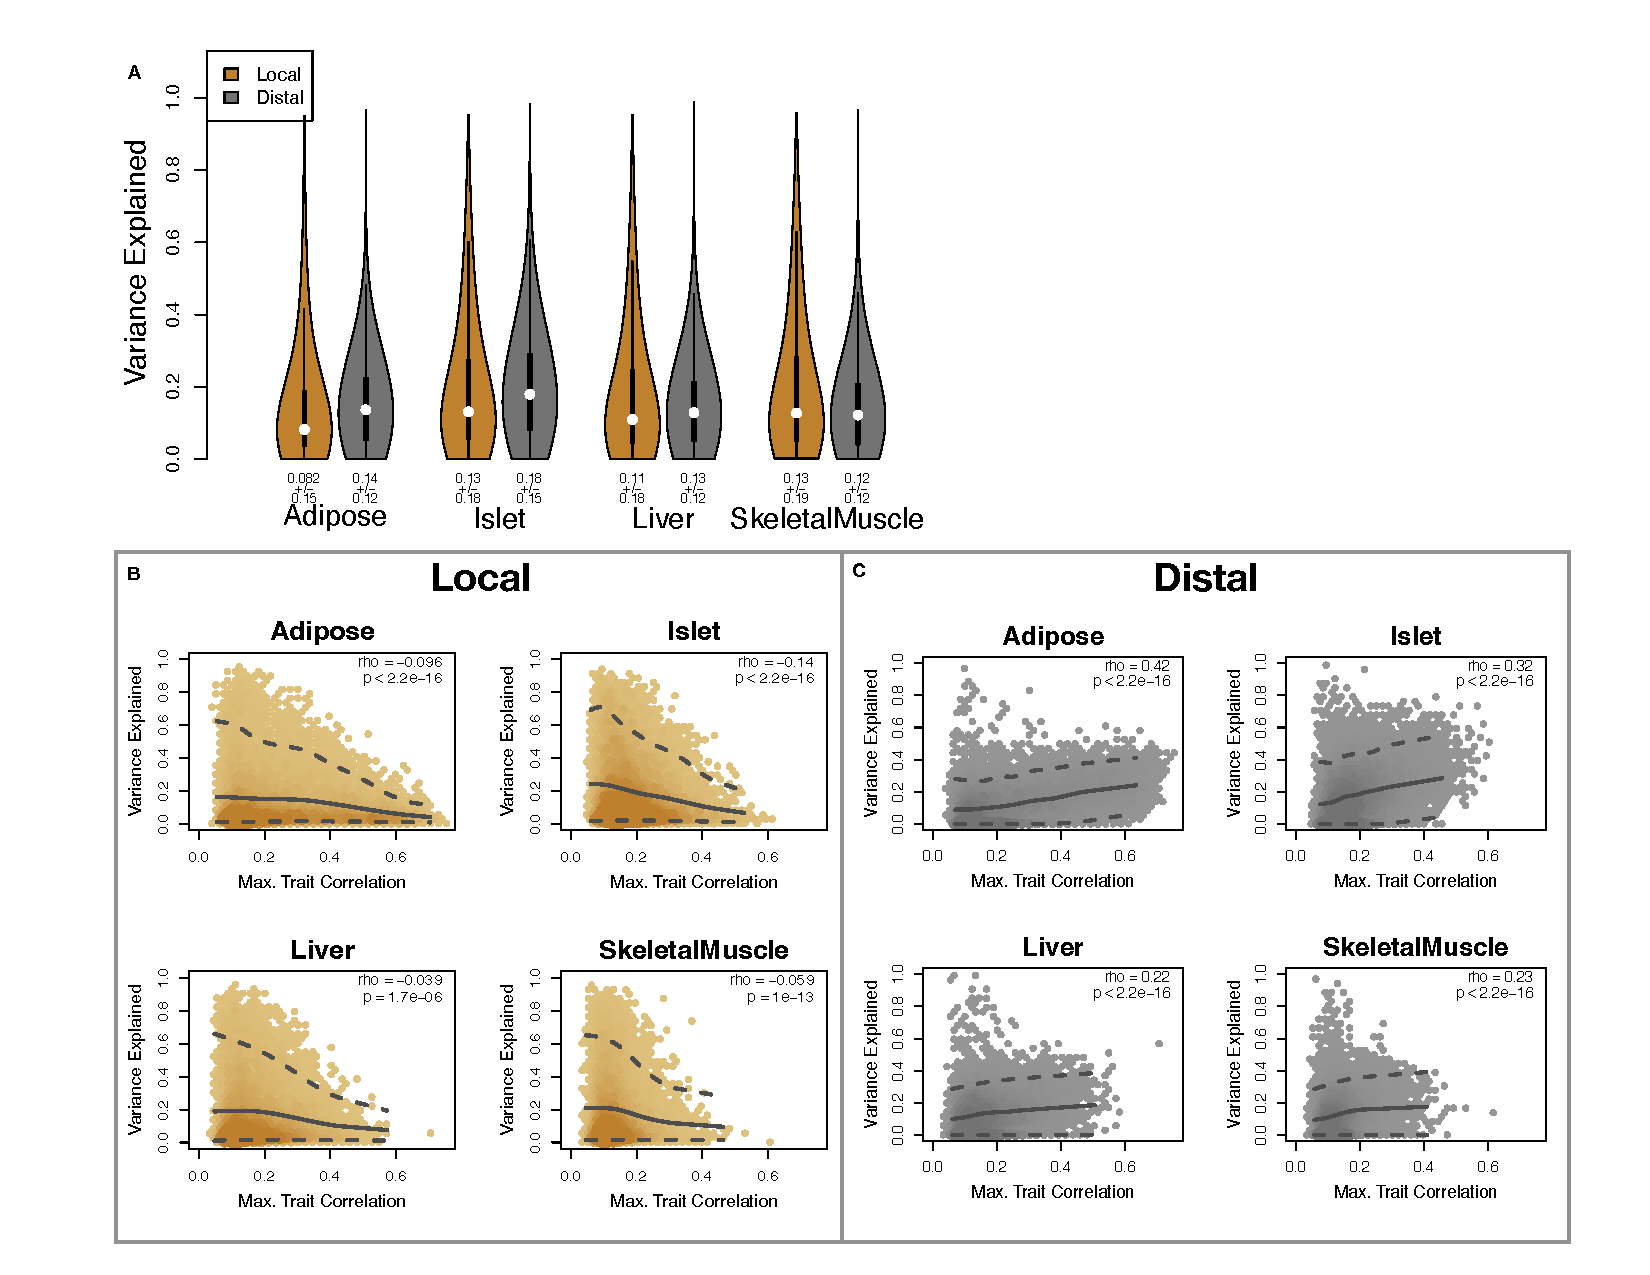
\includegraphics[width=\textwidth]{Figures/Fig2_motivation.pdf} 
\caption{Transcript heritability and trait relevance. 
\textbf{A.} Distributions of local (brown) and distal (gray) 
heritability of transcripts across the four tissues. Overall 
local and distal factors contribute equally to transcript 
heritability. Each distribution contains 14102 transcripts. 
Numbers below distributions indicate the median and 
standard deviation of each. \textbf{B.} local (brown) and 
\textbf{C.} distal (gray) heritability and trait relevance across 
all four tissues. Here trait relevance is defined as the maximum 
correlation between the transcript and all traits. The upper 
and lower dashed line in each panel show the 95th and 5th 
percentile correlation respectively. The solid line shows the 
mean trait correlation in transcripts with increasing variance 
explained either locally (B) or distally (C). Transcripts that are 
highly correlated with traits tend to have low local heritability 
and high distal heritability. All $p$ values from Spearman rank
correlation tests are two-sided. No adjustments were made 
for multiple comparisons. Source data are provided as a Source 
Data file.}
\label{fig:motivation}
\end{figure}

\begin{figure}[ht!]
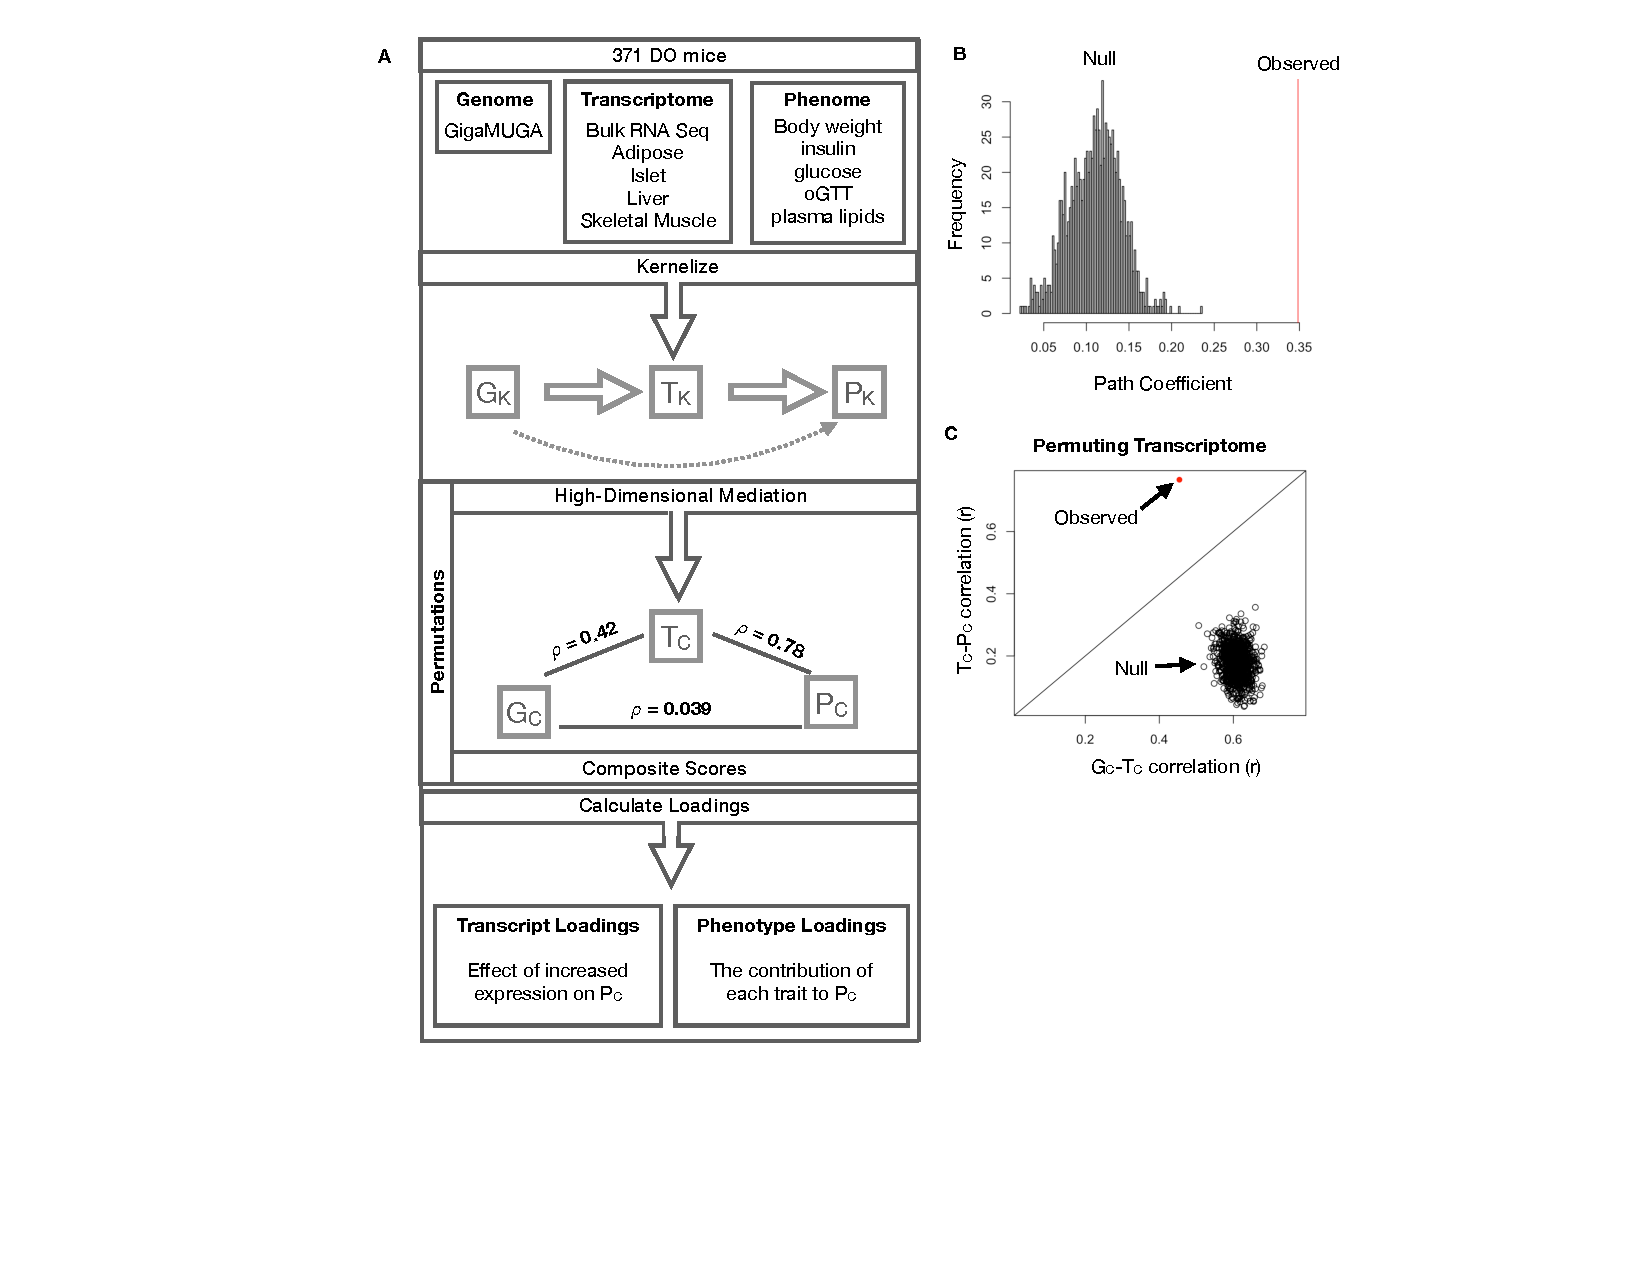
\includegraphics[width=5in]{Figures/Fig3_workflow.pdf} 
\caption{High-dimensional mediation. \textbf{A.} Workflow 
indicating major steps of high-dimensional mediation. The 
genotype, transcriptome, and phenotype matrices were 
kernelized to yield single matrices representing the 
relationships between all individuals for each data modality 
($G_K$ = genome kernel, $T_K$ = transcriptome kernel; 
$P_K$ = phenome kernel). High-dimensional mediation 
was applied to these matrices to maximize the direct path 
$G \rightarrow T \rightarrow P$, the mediating pathway 
(arrows), while simultaneously minimizing the direct $G 
\rightarrow P$ pathway (dotted line). The composite 
vectors that resulted from high-dimensional mediation 
were $G_c$, $T_C$, and $P_C$. The partial correlations 
$\rho$ between these vectors indicated perfect mediation. 
Transcript and trait loadings were calculated as described 
in the methods. \textbf{B.} The null distribution of the path 
coefficient derived from 10,000 permutations. Comparisons 
are shown to the observed path coefficient (red) the path 
coefficient using a distal-only model (gray) and the path 
coefficient using the local-only model (brown). \textbf{C.} 
The null distribution of the $G_C$-$T_C$ correlation vs. 
the $T_C$-$P_C$ correlation. Comparisons are shown 
to the observed values (red), and those derived from the 
distal-only model (gray) and the local-only model (brown).
Source data are provided as a Source Data file.
}
\label{fig:workflow}
\end{figure}

\begin{figure}[ht!]
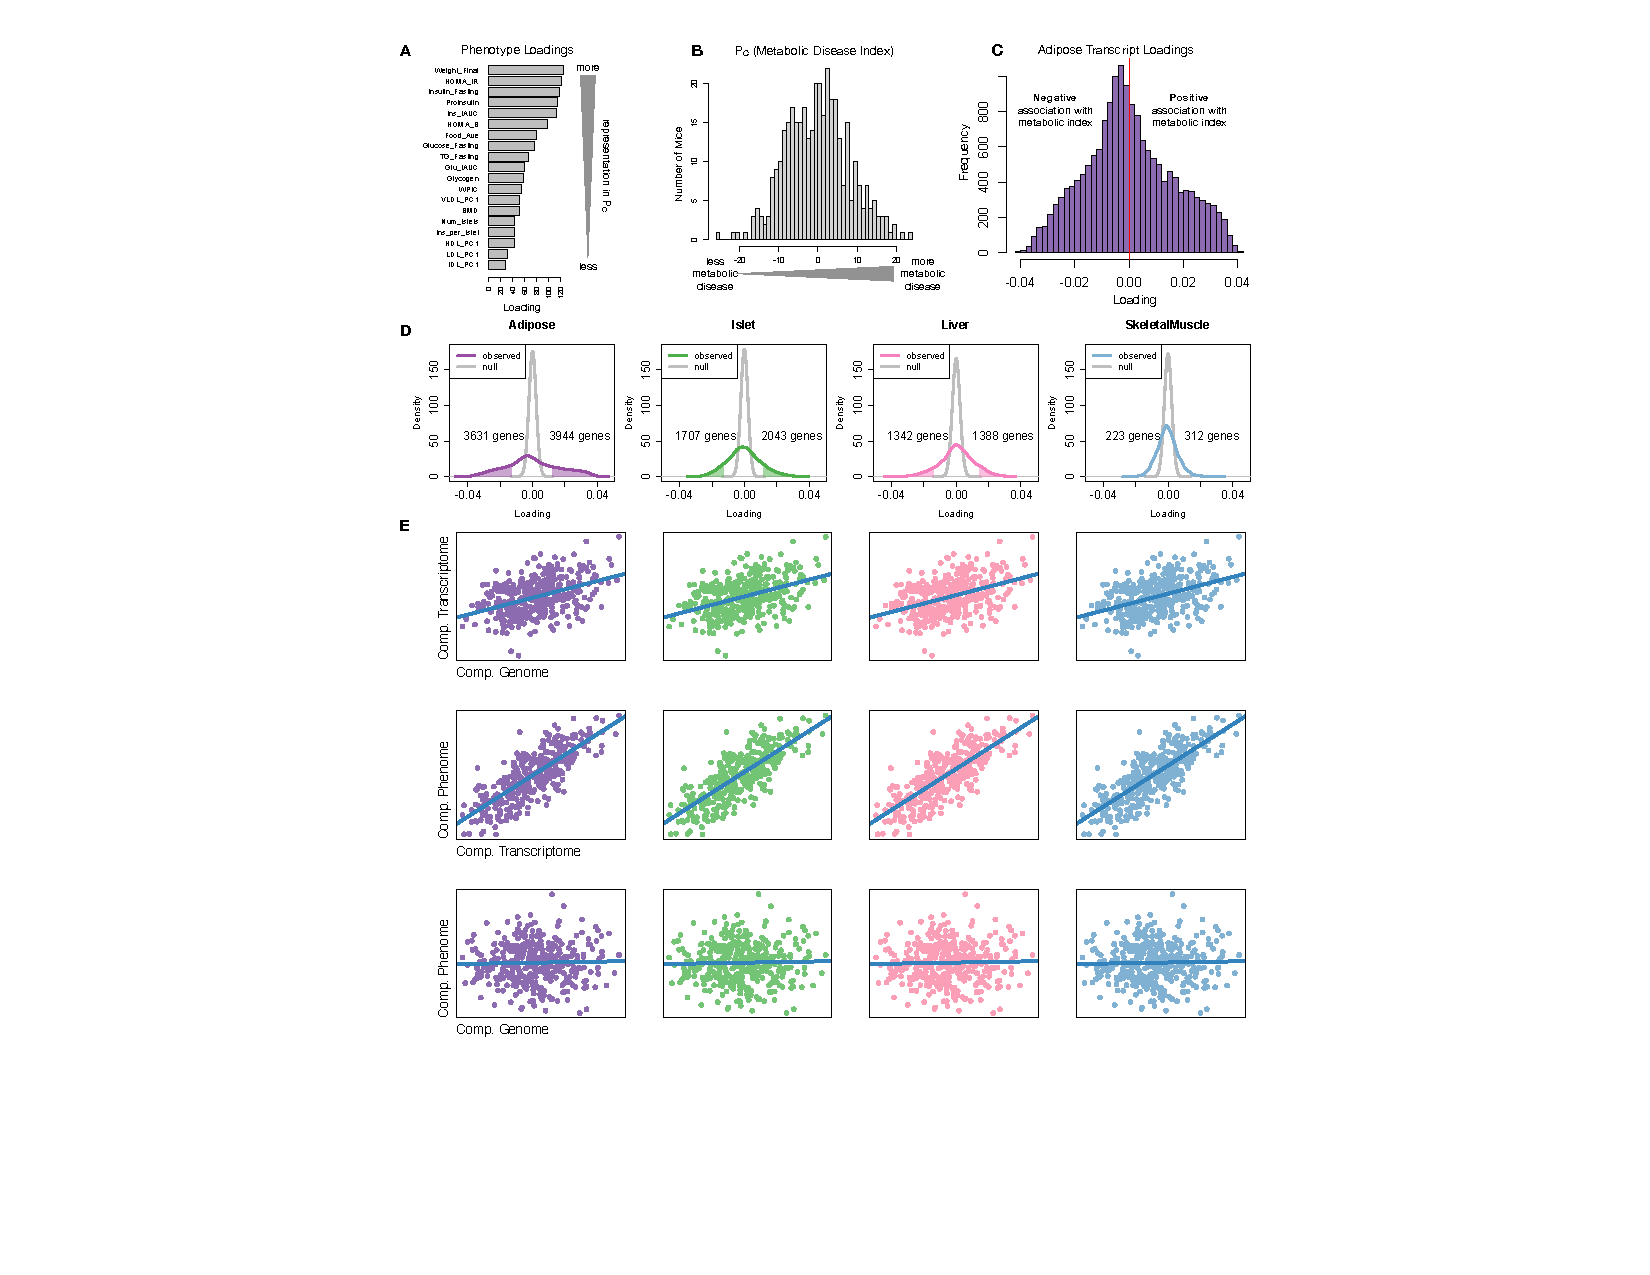
\includegraphics[width=\textwidth]{Figures/Fig4_interpretation.pdf} 
\caption{Interpretation of loadings. \textbf{A.} Loadings across traits. 
Body weight and insulin resistance contributed the most 
to the composite trait. \textbf{B.} Phenotype scores across 
individuals. Individuals with large positive phenotype scores 
had higher body weight and insulin resistance than average. 
Individuals with large negative phenotype scores had lower 
body weight and insulin resistance than average. \textbf{C.} 
Distribution of transcript loadings in adipose tissue (purple). 
For transcripts with large positive loadings, higher expression 
was associated with higher phenotype scores. For transcripts 
with large negative loadings, higher expression was associated 
with lower phenotype scores. \textbf{D.} Distributions of loadings 
across tissues compared to null distributions. Shaded areas 
represent loadings that were more extreme than the null 
distribution. Numbers indicate how many transcripts had loadings 
above and below the extremes of the null. Transcripts in adipose 
tissue (purple) had the most extreme loadings indicating 
that transcripts in adipose tissue were the best mediators of the 
genetic effects on body weight and insulin resistance. \textbf{E.} 
Scatter plots showing correlations between composite vectors for 
the genome ($G_C$), the transcriptome ($T_C$), and the phenome 
($P_C$). The $G_C$ - $T_C$ association was significant 
(Linear regression $R^2 = 0.18$;  beta coefficient = $7.8\pm0.86$ 
standard error; $t = 9.03$; $p < 2.2^{-16}$). The $T_C$ - $P_C$ 
association was significant (Linear regression $R^2 = 0.62$;  
beta coefficient = $3.1\pm0.13$ standard error; $t = 24.4$; 
$p < 2.2^{-16}$). There is no association between $G_C$ and $P_C$
(Linear regression $R^2 = 7.1\times10^{4}$;  beta coefficient = 
$2.0\pm3.8$ standard error; $t = 0.51$; $p = 0.61$). This correlation 
structure is consistent with perfect mediation. Blue lines show
lines of best fit. Source data are provided as a Source Data file.
}
\label{fig:interpretation}
\end{figure}

\begin{figure}[ht!]
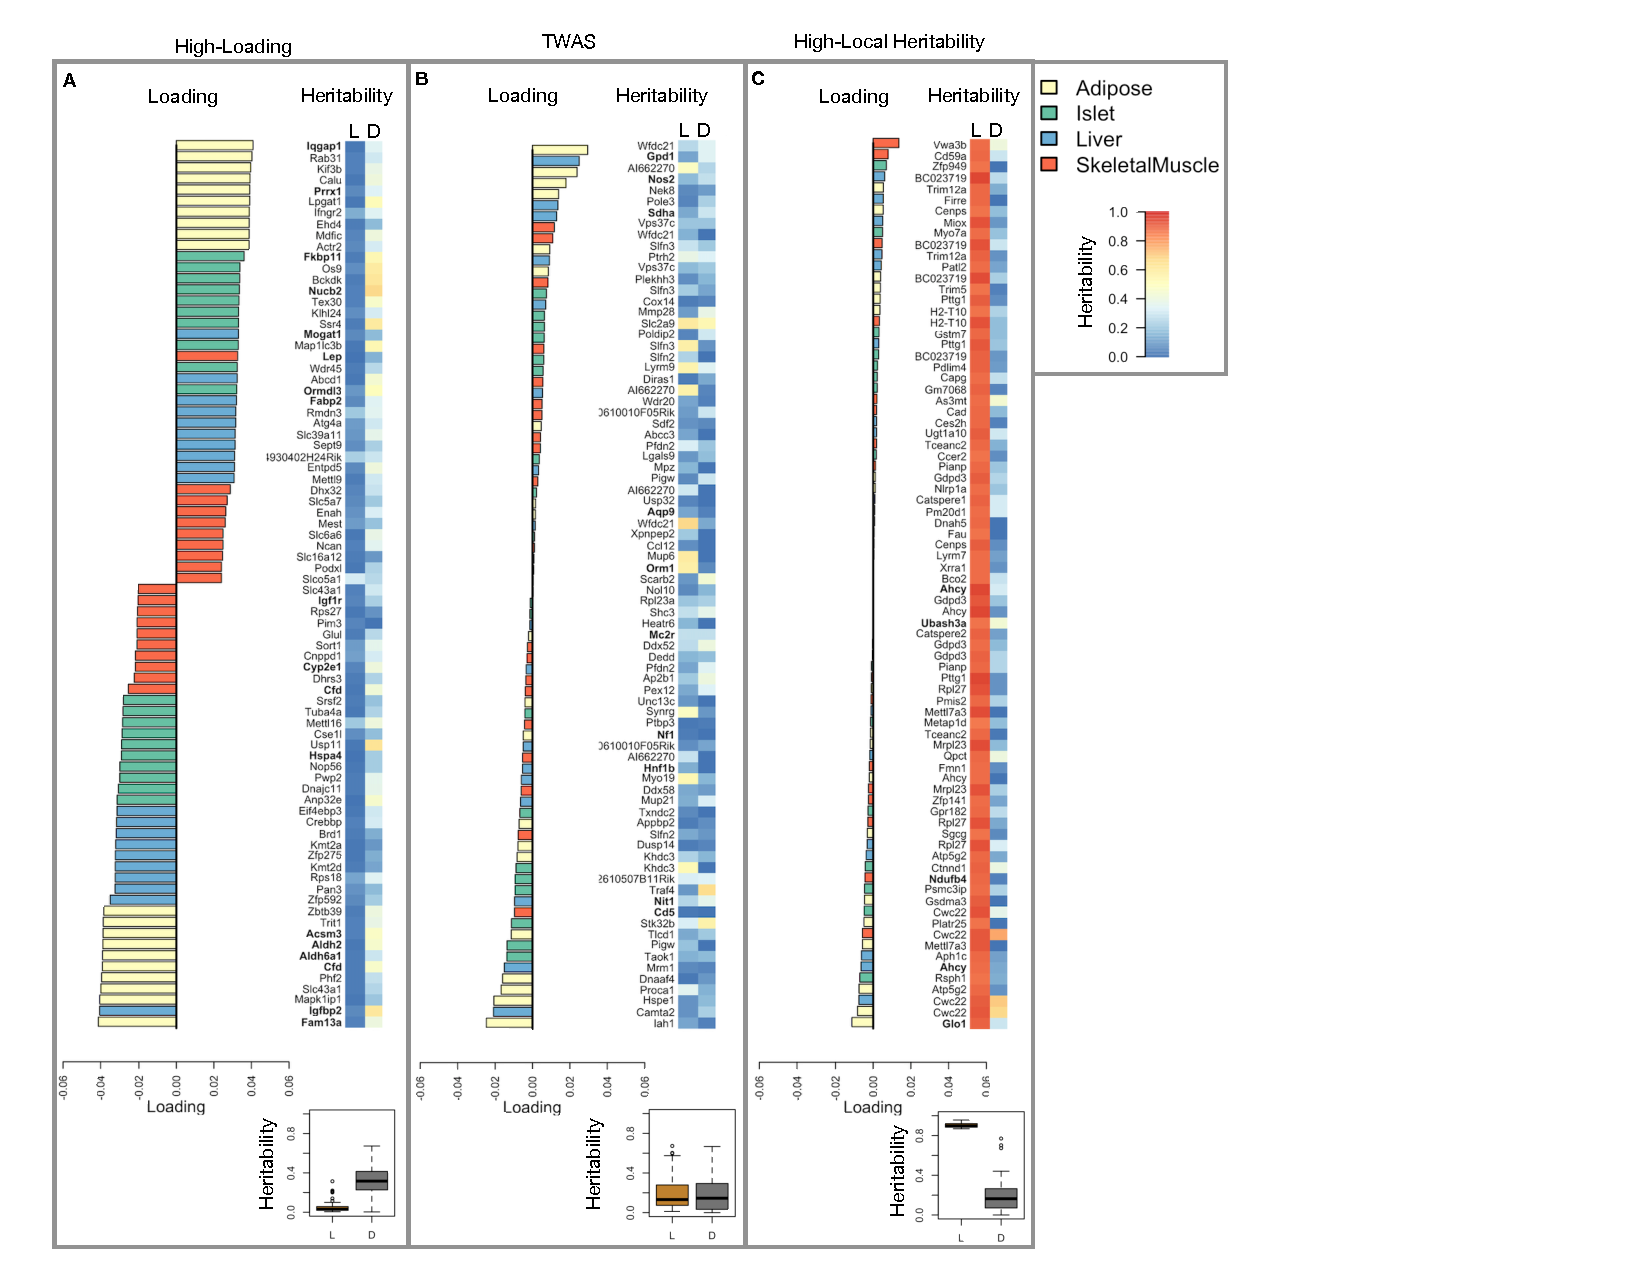
\includegraphics[width=\textwidth]{Figures/Fig5_loading_heritability.pdf} 
\caption{Transcripts with high loadings have high distal heritability 
and literature support. Each panel has a bar plot showing 
the loadings of transcripts selected by different criteria. 
Bar color indicates the tissue of origin. The heat map 
shows the local (L - left) and distal (D - right) heritability 
of each transcript. \textbf{A.} Loadings for the 10 
transcripts with the largest positive loadings and the 10 
transcripts with the largest negative loadings for each tissue. 
Mean distal heritability (31.8\%) was significantly higher than 
mean local heritability (5\%) (two-sided Welch's 
t-test $t = 16.4$; df = 100.2; difference 95\% CI = 0.24 to 
0.30; $p < 2.2^{-16}$). \textbf{B.} Loadings of TWAS 
candidates with the 10 largest positive correlations with 
traits and the largest negative correlations with traits across 
all four tissues. Mean local (15\%) and distal (20\%) heritability
were not significantly different for this group of transcripts 
(two-sided Welch's t-test $t = 1.9$; df = 151.7; difference 95\% 
CI = -0.002 to 0.1; $p = 0.77$). \textbf{C.} The transcripts 
with the largest local heritability (top 20) across all four 
tissues. Mean local heritability (90\%) was significantly higher 
than mean distal heritability (15\%) of these genes 
(two-sided Welch's $t = 45.0$; df = 82.0; difference 95\% 
CI = 0.72 to 0.78; $p < 2.2^{-16}$). Lines in boxes correspond 
to the median; lower and upper edges of boxes indicate the 
first and third quartiles; whiskers indicate the first and 
third quartiles $\pm$ 1.5 times the interquartile range; dots 
indicate outliers beyond 1.5 times the interquartile range. All 
$p$ values derived from two-sided Welch's t-test and are 
not adjusted for multiple comparisons. Source data are 
provided as a Source Data file.
}
\label{fig:loading_heritability}
\end{figure}

\begin{figure}[ht!]
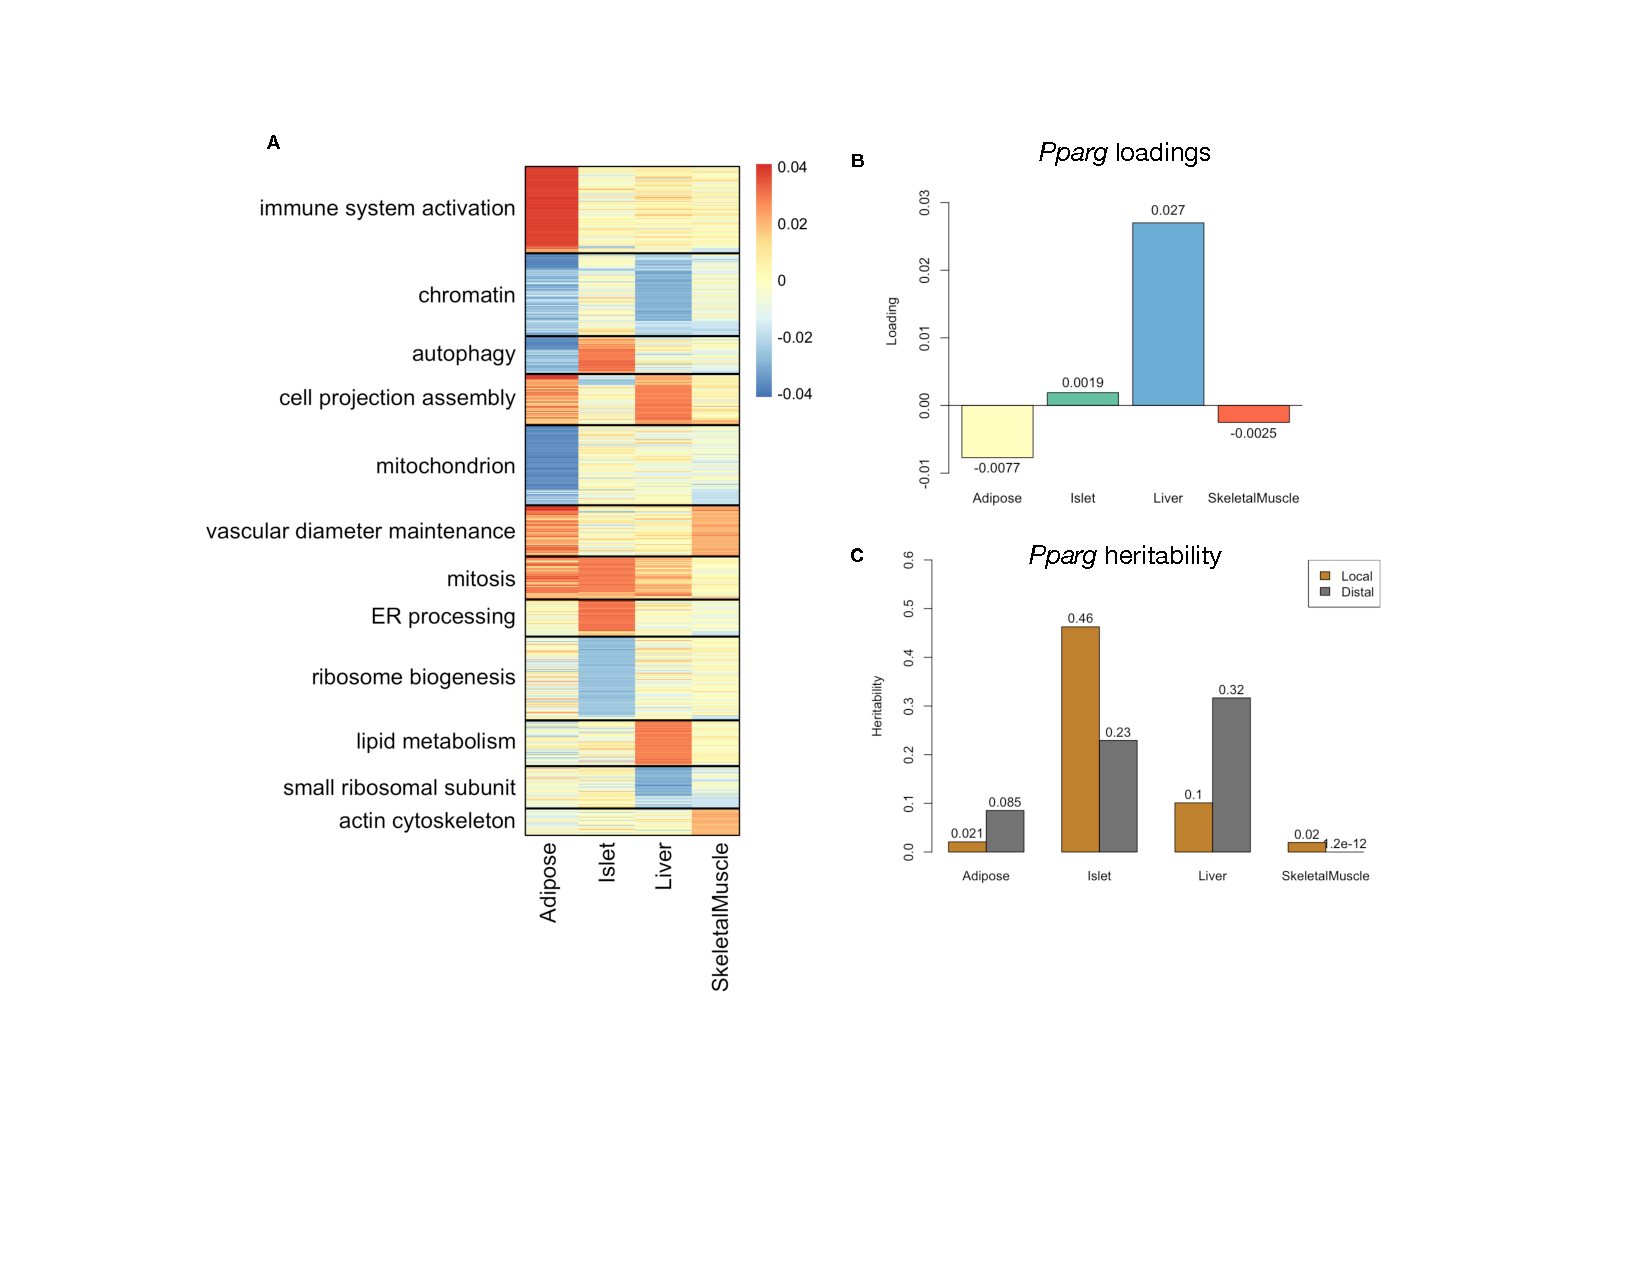
\includegraphics[width=\textwidth]{Figures/Fig6_TOA.pdf} 
\caption{Tissue-specific transcriptional programs are 
associated with obesity and insulin resistance. \textbf{A} 
Heat map showing the loadings of all transcripts with 
loadings greater than 2.5 standard deviations from the 
mean in any tissue. The heat map was clustered using 
$k$ medoid clustering. Functional enrichments of each 
cluster are indicated along the left margin. \textbf{B} 
Loadings for \textit{Pparg} in different tissues indicated 
by color. \textbf{C} Local (brown) and distal (gray) of 
\textit{Pparg} expression in different tissues. Source data 
are provided as a Source Data file.
}
\label{fig:toa}
\end{figure}

\begin{figure}[ht!]
\includegraphics[width=\textwidth]{Figures/Fig7_CC_Prediction.pdf} 
\caption{Transcription, but not local genotype, predicts 
phenotype in the CC-RIX. \textbf{A.} Workflow showing 
procedure for translating HDM results to an independent 
population of mice. \textbf{B.} Relationships between the 
predicted metabolic disease index (MDI) and the mean
of the rankZ normalized body weight. In this column,
MDI was derived from measured transcripts. Adipose - 
$R^2 = 0.60$;  beta coefficient = $0.89\pm0.17$ 
standard error; $t = 5.21$; $p = 5.9\times10^{-5}$.
Liver - $R^2 = 0.35$;  beta coefficient = $1.1\pm0.34$ 
standard error; $t = 3.1$; $p = 6.4\times10^{-3}$.
Muscle - $R^2 = 0.29$;  beta coefficient = $0.64\pm0.24$ 
standard error; $t = 2.7$; $p = 0.014$.
\textbf{C.} In this column, MDI was derived from 
transcripts imputed from local genotype. Adipose - 
$R^2 = 8.0\times10^{-4}$;  beta coefficient = $-0.2\pm0.16$ 
standard error; $t = -0.12$; $p = 0.91$.
Liver - $R^2 = 0.035$;  beta coefficient = $0.13\pm0.16$ 
standard error; $t = 0.81$; $p = 0.43$.
Muscle - $R^2 = 0.079$;  beta coefficient = $0.19\pm0.16$ 
standard error; $t = 1.24$; $p = 0.23$.
Gray boxes indicate measured quantities and blue boxes 
indicate calculated quantities. G - genome; T - transcriptome; 
P - phenome (here MDI). The dots in each panel represent 
individual CC-RIX strains. Each strain was represented 
by between 19 and 24 individuals. The gray lines show 
the standard deviation of mean body weight for the 
strain. Source data are provided as a Source Data 
file.
}
\label{fig:cc_prediction}
\end{figure}

\begin{figure}[ht!]
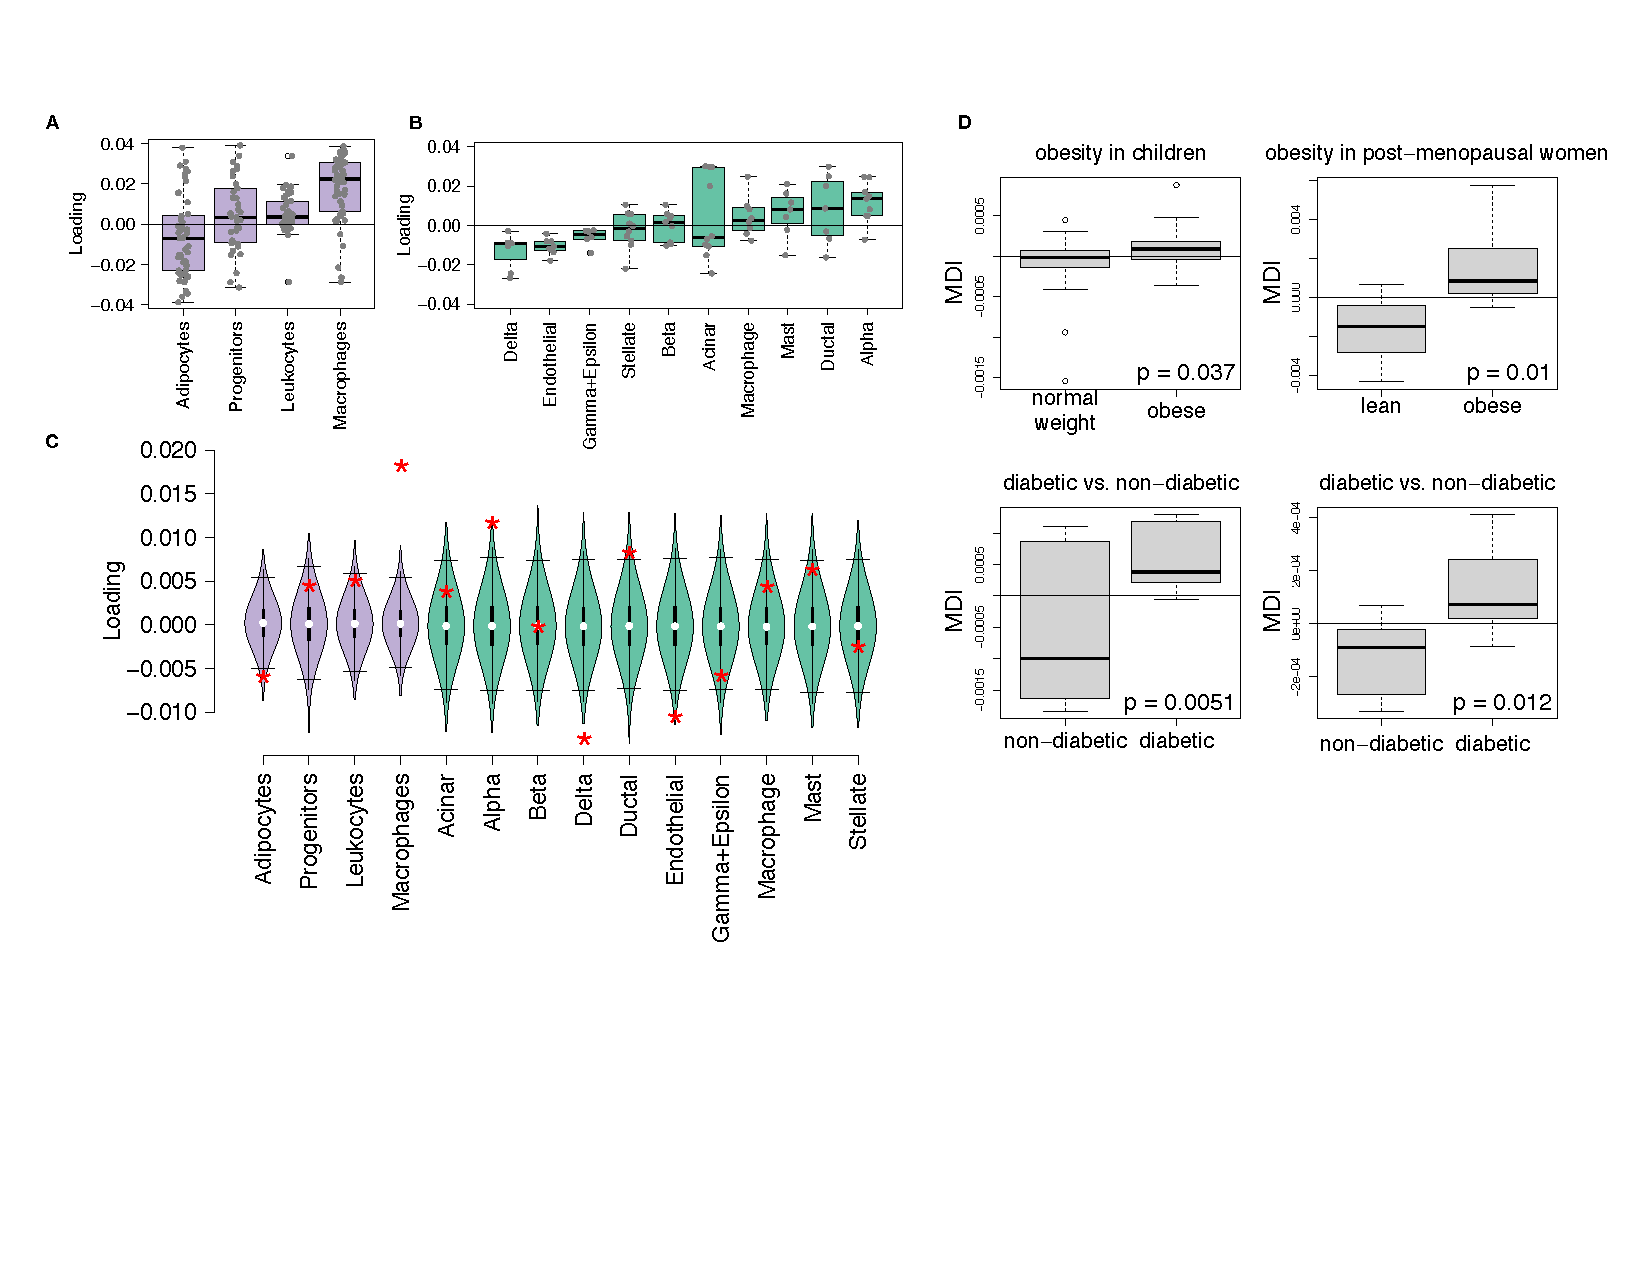
\includegraphics[width=\textwidth]{Figures/Fig8_Human_Translation.pdf} 
\caption{HDM results translate to humans. \textbf{A.} Distribution of 
loadings for cell-type-specific transcripts in adipose tissue
(purple). Numbers in parentheses indicate the number of 
transcripts in each group. \textbf{B.} Distribution of loadings 
for cell-type-specific transcripts in pancreatic islets (green). 
Each box in this panel represents 10 transcripts. \textbf{C.} 
Null distributions from 10,000 permutations for the mean 
loading of randomly selected transcripts in each cell type 
compared with the observed mean loading of each group 
of transcripts (red asterisk). Violin plot colors indicate the 
tissue of each cell type and match panels A and B 
(purple = adipose; green = islet) \textbf{D.} Predictions of 
metabolic disease index (MDI) in four adipose transcription 
data sets downloaded from GEO. In each study the 
obese/diabetic patients were predicted to have greater 
MDI than the lean/non-diabetic patients based on the 
HDM results from DO mice. 1) two-sided Welch's $t$ test: $t = 2.28$, 
df = 58.1, 95\% CI of difference = $2.1\times10^{-5}$ 
to $3.2\times10^{-4}$ A.U.; $p = 0.027$
2) two-sided Welch's $t$ test: $t = 3.04$, 
df = 11.84, 95\% CI of difference = $9.3\times10^{-4}$ 
to $5.7\times10^{-3}$ A.U.; $p = 0.01$
3) linear mixed effects model: 
fixed effect diabetic = 
$1.4\times10^{-3}\pm5.6\times10^{-4}$ Std. Error;
$t = 2.4$, df = 4, $p = 0.075$
4) two-sided Welch's $t$ test: $t = 2.95$, 
df = 11.89, 95\% CI of difference = $6.8\times10^{-5}$ 
to $4.6\times10^{-4}$ A.U.; $p = 0.012$
Lines in boxes correspond to the 
median; lower and upper edges of boxes indicate the 
first and third quartiles; whiskers indicate either the minimum
and maximum values if no outliers, or the first and third quartiles 
$\pm$ 1.5 times the interquartile range if there are outliers; 
dots indicate outliers beyond 1.5 times the interquartile range. 
The number of patients in each group is indicated by numbers 
in parentheses with the number of technical replicates (reps) if 
relevant. No adjustments were made for multiple comparisons. 
Source data are provided as a Source Data file.
}
\label{fig:human_translation}
\end{figure}

\end{document}
